\chapter{Propagating the uncertainty of stereo images}
This chapter details the work conducted on the propagation of uncertainty from images into the cost curves of dense matching problems. We consider a simple model of uncertainty on the input images, a dependency model between the uncertain intensities of the images, and estimate the resulting uncertainty on the output cost curves. This chapter takes up work and data already published \cite{malinowski_copulas_2022, malinowski_uncertainty_2023, malinowski_robust_2024}.

\section{Sources of uncertainty in stereo matching}
\comroman{Maybe move this section after having presented the different ways to use Copulas and IP. 
Atmospheric correction, vibration, resolution of a pixel, discretization.
CO3D mission will not have the epipolar line correction problem that is encountered with pleiades images.
Epipolar line rectification for Pléiades is a problem that is not dealt here.}

To maintain simplicity in this section, we will not consider panchromatic images, such as Pléiades products, encoding the reflectance values as positive integer, usually contained in $[0, 5000]$. Instead, we consider grayscale images that have intensity levels quantified within the range $[0, 255]$, which will represent our measurable space $\X$. We hypothesize that a pixel's intensity value can deviate by no more than $1$ level from its observed value, with the observed value being the most likely. This hypothesis arises from the quantification of observed radiometric values into integers. To keep our explanation straightforward, we assume this simple hypothesis. Consequently, we model the uncertainty of each pixel $p\in I_L,I_R$ intensity with a possibility distribution $\pi$, centered around the observed intensity $i_p\in[0,255]$:
\begin{equation}
    \pi(i_p)=1,\quad \pi(i_p\pm1)=\alpha\,,
\end{equation}\label{eq:pixel_possibility}
with $\alpha \in [0,1]$. The $\pm$ indicates that both positive and negative values are considered. In our simulation, $\alpha = 0.3$ for pixels in the left image and $\alpha = 0.4$ for pixels in the right image. We use different values of $\alpha$ for the left and right images because the uncertainty model may vary between images due to differences in exposure, noise levels, or camera calibration. This model effectively states that we accept any probability distribution supported within $[i_p - 1, i_p + 1]$ where the probability measure $P$ satisfies $\{P(A) \leq \sup_{i \in A} \pi(i)\}$ as an acceptable model for our uncertainty. The mass distribution function $m_p$ associated to this credal set possesses two focal sets $a^p$:
\begin{eqnarray}
    &m_p(a^p_1=[\![i_p, i_p]\!])=1-\alpha\,\nonumber\\
    &m_p(a^p_2=[\![i_p-1, i_p + 1]\!])=\alpha\,\label{eq:pixel_mass}
\end{eqnarray}
with $[\![\cdot, \cdot]\!]$ referring to integer intervals. In particular, $[\![i_p, i_p]\!]$ correspond to the singleton $\{i_p\}$.

It is important to note that in this disparity estimation problem, we only account for the uncertainty in our input image intensities, without considering the uncertainty in our cost function's ability to correctly identify the true disparity as its minimum. In other words, we do not account for the uncertainty arising from the difference between ``two patches are very similar'' and ``the pixels at the center of the patches are homologous''. To better illustrate this, imagine a scenario where two pixels should be matched, but the surrounding patches are dissimilar. In this case, the cost function between those two patches would be high, potentially leading to the selection of a different patch with a lower cost function as the estimated disparity. The correct disparity would not be the minimum of the cost curve.

\section{Methods for Joining credal sets with copulas}
When working with multiple sources of uncertain information, one must take into account the dependency between the different sources in order to correctly determine the joint model. Section \ref{sec:copulas} introduced copulas, a type of dependency model that we will be using for joining the uncertainty model on images intensities. We consider here $n\in\mathbb{N}^*$ uncertain variables $(X_i)_{1\leqslant i\leqslant n}$ taking values respectively in an totally ordered finite space $\X_i$. Index $i$ will usually refer to the $i$-th random variable (or random set). We note $\M_i$ the credal set representing the uncertainty of $X_i$, and $C$ a $n$-copula. Focal sets of a belief function will be noted $a^i_k$, where $k$ refers to the $k$-th focal set if they are numbered. We also note $\bigsqcup$ the union of disjoint elements.

When working with precise probabilities, a copula $C$ joins univariate Cumulative Distribution Functions (CDF), called marginals, into a mutlivariate CDF. When working with marginals modeled by Imprecise Probabilities, joining the models with a copula on the product space $\X=\X_1\tdt\X_n$ is not as straightforward. We present here three different approaches to create a multivariate credal set using a copula and imprecise marginals. 

\subsection{Point-wise aggregation}
A first way of creating a joint credal set is to sample a precise marginal for each marginal credal sets $\M_i$ and to use Sklar's theorem with the copula $C$ to create a precise multivariate CDF. The set of all resulting CDFs is thus:
\begin{eqnarray}\label{eq:robust_ancestor}
    \mathcal{S}(C,\M_i) = \{F~|~\forall x_i \in \X_i,~ F(x_1,\dots,x_n) = C(F_1(x_1), \dots, F_n(x_n))\}
\end{eqnarray} where $F_i\in\M_i$.

This set is not strictly a credal set as it is not guaranteed to be convex \cite{schmelzer_random_2023}. We thus define the joint credal set as the convex hull $\M_{robust}$ of $\mathcal{S}$:

\begin{eqnarray}\label{eq:robust_set}
    \M_{robust}(C,\M_i) = \{&&F~|~\forall A \in \X,\nonumber\\
    &&\inf_{G\in\mathcal{S}(C,\M_i)}G(A)\leqslant F(A)\leqslant\sup_{G\in\mathcal{S}(C,\M_i)}G(A)~\}
\end{eqnarray}

We refer to this joint credal set as $\M_{robust}(C,\M_i)$ as it contains every element of the marginal credal sets with copula $C$ as their dependency model. We will omit ``$(C,\M_i)$'' when there are no confusion possible to avoid using heavy notations. $\M_{robust}$ is thus the smallest credal set containing $\mathcal{S}$. It is interesting to notice that it can contain additional multivariate CDFs that do not possess the copula $C$ as the dependency model of its marginals. This credal set is not easy to compute for events that are not Cartesian products of marginal cumulated events

\subsection{Copula applied to cumulated mass functions}
In this section, we will present another way of creating a joint credal set from multiple marginal ones. Consider the same copula $C$ as before and the same marginal credal sets $\M_i$. Each credal set $\M_i$ is fully determined by a mass distribution function $m_i$, which is strictly positive over its $N_i$ focal sets $a^i_1, \dots, a^i_{N_i}$. As described in \cite{ferson_dependence_2004}, it is possible to use the cumulated mass distribution functions as marginals of the copula to create a joint mass distribution function, granted that there is a complete order defined on the focal sets. Links between copulas and belief functions have been investigated in the continuous case in \cite{schmelzer_joint_2015, schmelzer_multivariate_2019}, the special case of necessity functions in \cite{schmelzer_sklars_2015} and of p-boxes in \cite{schmelzer_random_2023}.

Let suppose, without loss of generality, that the marginal focal sets are numbered according to the order $\preceq_i$: $a^i_1\preceq_ia^i_2\preceq_i\dots\preceq_i a^i_{N_i}$. The idea behind this method is to replace the precise marginal CDFs by cumulated masses, to conserve the philosophy behind Sklar's theorem. We thus first define the joint mass $m_\times$ on the product space of focal sets. Let $a_{k_i}^i$ be the $k_i$-th focal set of $m_i$ according to the chosen order. $m_\times$ is computed as the H-volume of copula $C$ computed over the cumulated marginal masses:
\begin{eqnarray}\label{eq:joint_mass}
    m_\times(a^1_{k_1}\tdt a^n_{k_n}) = H_{\sum_{k=0}^{k_1-1}m_1(a^1_k), \dots, \sum_{k=0}^{k_n-1}m_n(a^n_k)}^{\sum_{k=0}^{k_1}m_1(a^1_k), \dots, \sum_{k=0}^{k_n}m_n(a^n_k)}
\end{eqnarray}
with the convention that $\forall i, a^i_0=\emptyset$, which is not strictly a focal set but allows to deal with the case $k_i=1$ as $m_i(a^i_0)=0$. For sets that are not of the form $a^1_{k_1}\tdt a^n_{k_n}$, the mass $m_\times$ is null. By this definition, $m_\times$ is a correctly defined mass distribution function.
\begin{proof}
    By definition it holds that $m_\times(\emptyset)=0$, and the properties of the H-volume impose that $m_\times\in[0,1]$.
    
    There are multiple way of proving that $\sum_{A\subseteq\X}m_\times(A)=1$. A direct proof can be done in the case $n=2$, but the notations become quite for any $n>2$. Instead let us use the interpretation of a copula as a multivariate CDF. 
    Let $\forall i\in[\![0, n]\!], F_i$ be a CDF over $[0, N_i]$, with ,$~F_i(j)=\sum_{k=0}^j m_i(a_k^i)$. By Sklar's theorem, $F=C(F_1,\dots, F_n)$ is a multivariate CDF over $[0, N_1]\tdt[0, N_n]$. Thus it holds that $F([0, N_1]\tdt[0, N_n])=1$ and:
    \begin{eqnarray*}
        F([0, N_1]\tdt[0, N_n]) &=& F([0,\dots,0])+\\
        &&F\left(\bigsqcup_{k_1=0}^{N_1-1}\dots\bigsqcup_{k_n=0}^{N_n-1}\left(]k_1, k_1+1]\tdt]k_n, k_n+1]\right)\right)\\
        &=& 0 + \sum_{k_1=0}^{N_1-1}\dots\sum_{k_n=0}^{N_n-1} F(]k_1, k_1+1]\tdt]k_n, k_n+1])\\
        && \text{(CDF of an union of disjoint elements)}\\
        &=& \sum_{k_1=0}^{N_1-1}\dots\sum_{k_n=0}^{N_n-1} H_{F_1(k_1), \dots, F_n(k_n)}^{F_1(k_1+1), \dots, F_n(k_n+1)}\\
        &=& \sum_{k_1=1}^{N_1}\dots\sum_{k_n=1}^{N_n} H_{\sum_{k=0}^{k_1-1}m_1(a^1_k), \dots, \sum_{k=0}^{k_n}m_n(a^n_k)}^{\sum_{k=0}^{k_1}m_1(a^1_k), \dots, \sum_{k=0}^{k_n}m_n(a^n_k)}\\
        &=& \sum_{(a^1_{k_1}\tdt a^n_{k_n})\subseteq\X}m_\times(a^1_{k_1}\tdt a^n_{k_n})
    \end{eqnarray*}
Therefore it holds that:
\begin{eqnarray}
    \sum_{A\subseteq\X}m_\times(A)=\sum_{(a^1_{k_1}\tdt a^n_{k_n})\subseteq\X}m_\times(a^1_{k_1}\tdt a^n_{k_n})=1
\end{eqnarray}
which proves that $m_\times$ is a mass distribution function.
\end{proof}

Having defined a mass distribution function on the product space $\X$, we thus define the joint credal set $\M_{mass}$ as: 
\begin{eqnarray}\label{eq:credal_set_mass}
    \M_{mass} = \{P~|~\forall A\subseteq\X, P(A)\geqslant \sum_{a\subseteq A}m_\times(A)\}
\end{eqnarray}

With this way of defining the multivariate mass, the choice of arbitrary orders $\preceq_i$ can have a significant impact on the value of the multivariate mass function. The next example illustrate this statement.

\begin{example}\label{ex:joint_mass}
    Let us present an example in the case $n=2$. Let $m_1$ be a mass distribution function over the power set $\X_1$ with two focal sets $a_1, a_2$. Similarly, let $m_2$ be a mass distribution function over the power set $\X_2$ with two focal sets $a_1^2,~a_2^2$. Throughout this example we will assume that $a_1^2\preceq_2a_2^2$. We consider the minimum copula $C(u,v)=\min(u,v)$ and $m_1(a_1^1)=m_1(a_2^1)=m_2(a_1^2)=0.5$.
    If there is no natural order on the focal sets of $m_1$, we have to chose an arbitrary one:
    \begin{itemize}
        \item[-] If "$a_1^1\preceq_1a_2^1$" is the arbitrary order (see figure \ref{fig:joint_distrib_arb}), then
        \begin{eqnarray*}
            m_\times(a_1^1,~a_1^2) &=& C(m_1(a_1^1),~m_2(a_1^2))\\
            &=& 0.5\\
            m_\times(a_2^1,~a_1^2) &=& C(1,~m_2(a_1^2)) - C(m_1(a_1^1),~m_2(a_1^2))\\
            &=& m_2(a_1^2) - C(m_1(a_1^1),~m_2(a_1^2))\\
            &=& 0
        \end{eqnarray*}
        \item[-] If "$a_2^1\preceq_1a_1^1$" is the arbitrary order, then
        \begin{eqnarray*}
            m_\times(a_1^1,~a_1^2) &=& C(1,~m_2(a_1^2)) - C(m_1(a_2^1),~m_2(a_1^2))\\
            &=& m_2(a_1^2) - C(m_1(a_2^1),~m_2(a_1^2))\\
            &=& 0\\
            m_\times(a_2^1,~a_1^2) &=& C(m_1(a_2^1),~m_2(a_1^2))\\
            &=& 0.5
        \end{eqnarray*}
    \end{itemize}
    This illustrates that different orders lead to different masses and thus to different credal sets.
    \begin{figure}[!ht]
        \centering
        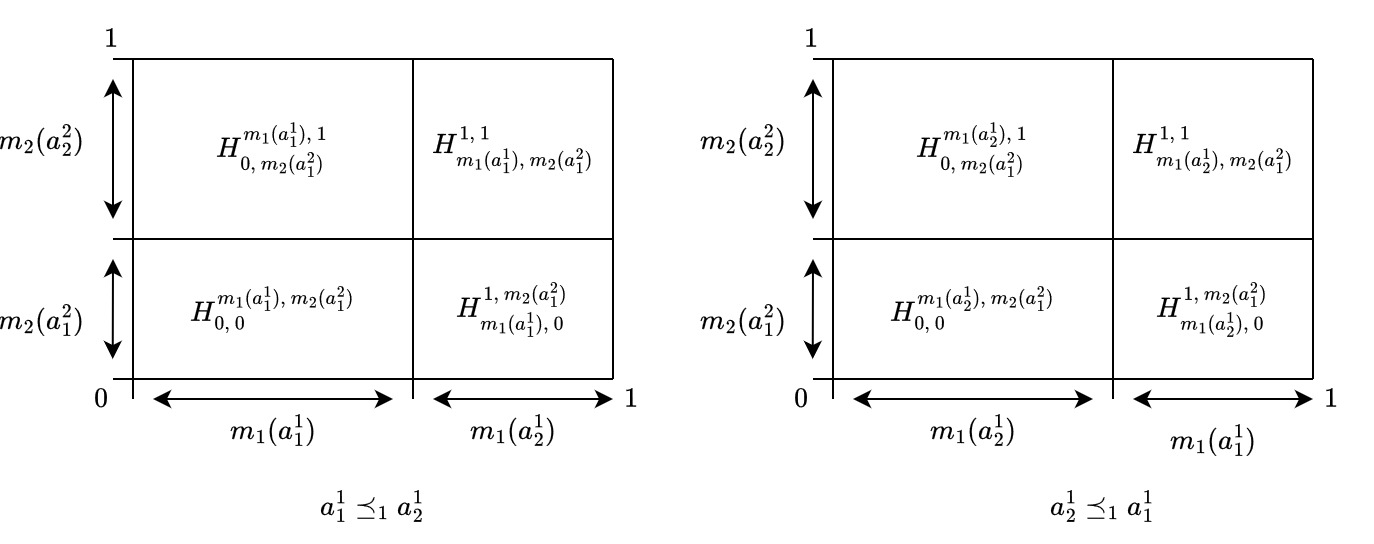
\includegraphics[width=\linewidth]{Images/M_mass_h_volume.jpg}
        \caption{H-volume diagram in the case $a_1^1\preceq_1a_2^1$}
        \label{fig:joint_distrib_arb}
    \end{figure}
\end{example}

In general, no order exists on the focal sets of belief functions, therefore an order has to be chosen arbitrarily. However, special cases of belief functions exhibit a natural order on their focal sets, for instance p-boxes and possibilities:
\begin{itemize}
    \item Focal sets of p-box are of the shape $a_\alpha = [\overline{F}^{-1}(\alpha),~\underline{F}^{-1}(\alpha)]$ (\cite{destercke_unifying_2008}), with $\alpha\in [0,1]$ and $F^{-1}$ being the inverse of a CDF (or quasi-inverse if the inverse does not exists). Thus the natural order for a p-box is $a_\alpha\preceq a_\beta \Leftrightarrow \alpha\leqslant\beta$
    \item Focal sets of possibility distributions form a nested family of sets. The natural order between the focal sets is therefore $a_1\preceq a_2 \Leftrightarrow a_1 \subseteq a_2$.
\end{itemize}

The credal set $\M_{mass}$ is different from $\M_{robust}$ as its bounds do not always coincide. This is because applying the copula to the cumulated masses instead of the CDFs encodes the correlation between sets and not between the underlying values of those sets, as it is usually done in the precise case. For instance, consider the setting of example \ref{ex:joint_mass} with $a_2^1\preceq_1a_1^1$, and suppose that the values covered by $a^1_1$ are high values in $\X_1$, and conversely that the values covered by $a^2_1$ are low values in $\X_2$. Applying the minimum copula to the cumulated masses would assign a null joint mass to $a_1^1\times a_1^2$. In the precise setting, joining two random variables in $\mathbb{R}$ with the minimum copula means that low values of the variables are positively correlated.

\subsection{Copulas applied to belief functions}
Another way of joining credal sets with a copula is by directly applying the copula to their lower envelope $\low_i$ for every event:
\begin{eqnarray}\label{eq:copula_on_lower_proba}
    \M_{agg} = \{P~|~\forall A_i\in\X_i, P(A_1,\dots, A_n)\geqslant C(\low_1(A_1), \dots, \low_n(A_n)\}
\end{eqnarray}

The constraints on this set only occur on the product space $\X_1\tdt \X_n$, contrary to $\M_{mass}$. We note $\M_{agg}$ this credal set as it uses the copula as an aggregation operator only, without conserving the meaning associated to copulas by Sklar's theorem. In this regard, $\M_{agg}$ has less meaning than $\M_{robust}$ or $\M_{mass}$, but presents the advantage of being easier to compute than those joint credal sets. Figure \ref{fig:meaning_computation} sums up the performances of the different methods in terms of computation cost and meaningfulness.

\begin{figure}[!hb]
    \centering
    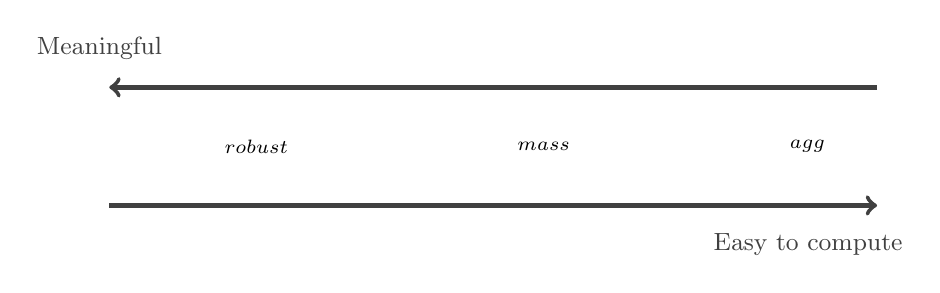
\begin{tikzpicture}[scale=1]
        \draw (0, 0) node (a) {};
        \draw (10, 0) node (b) {};
        \draw (0, 1.5) node (c) {};
        \draw (10, 1.5) node (d) {};
        
        \draw[->, ultra thick, darkgray] (a) to node[midway, left, inner sep=0.5cm] {} (b);
        \draw[->, ultra thick, darkgray] (d) to node[midway, left, inner sep=0.5cm] {} (c);
        
        \draw [darkgray] (9, -0.5) node (z) {\small Easy to compute};
        \draw [darkgray] (0, 2) node (z) {\small Meaningful};
        
        \draw (9, 0.75) node (z) {$\M_{agg}$};
        \draw (5.65, 0.75) node (z) {$\M_{mass}$};
        \draw (2, 0.75) node (z) {$\M_{robust}$};
    \end{tikzpicture}
    \caption{Comparing different methods of joining credal sets with a copula.}
    \label{fig:meaning_computation}
\end{figure}

In general, applying the copula directly to the lower probabilities as in (\ref{eq:copula_on_lower_proba}) does not produce a coherent lower probability that avoid sure loss. For instance, let us consider $\X_1 = \X_2 = \{1, 2\}$, two lower previsions $\low_1$ and $\low_2$ such that $\low_1(\{1\}) = \low_1(\{2\}) = \low_2(\{1\}) = \low_2(\{2\}) = 0.5$. Joining those two lower probabilities using the minimum copula $C(u,v)=\min(u,v)$ gives a mapping $\low$ which is neither coherent nor avoid sure loss (Table \ref{tab:non_coherent_lower}).

\begin{table}[!ht]
    \centering
    \begin{tabular}{|c||c|c|}
        \hline
        \hspace{0.2cm} $\low$ \hspace{0.2cm} & \hspace{0.2cm} $\{1\}$ \hspace{0.2cm} & \hspace{0.2cm} $\{2\}$ \hspace{0.2cm} \\\hline\hline
        $\{1\}$ & $0.5$ & $0.5$ \\\hline
        $\{2\}$ & $0.5$ & $0.5$\\
        \hline
        \end{tabular}
        \caption{$\low = \min(\low_1, \low_2)$}
        \label{tab:non_coherent_lower}
\end{table}

In the special case of the product copula $C_\Pi$, the joint lower probability $\low_{C_\Pi}$ induced by (\ref{eq:copula_on_lower_proba}) avoids sure loss if its marginals also avoid sure loss. It follows that for all copulas $C$ dominated by the product copula (\ie $C_\Pi\geqslant C$), and for every $\M_i$ avoiding sure loss, $\M_{agg}(C, \M_i)$ is a non empty credal set.
\begin{proof}
    For $i\in\{1,\dots,n\}$, let $\low_i$ be a lower probability avoiding sure lost, \ie whose credal set $\M_i$ contains at least one probability distribution $P_i$. Let us define a multivariate probability $P$ on every $(A_1\tdt A_n)\subseteq\X$ as:
    \begin{eqnarray*}
        P(A_1\tdt A_n) = P_1(A_1)\tdt P_n(A_n)
    \end{eqnarray*}
    Defining $P$ on $(A_1\tdt A_n)\subseteq\X$ is sufficient as those sets contain every atom of $\X$.
    Because $\forall i, P_i\in\M_i,~P_i\geqslant \low_i$, then:
    \begin{eqnarray*}
        P(A_1\tdt A_n) \geqslant \low_1(A_1)\tdt \low_n(A_n) &=& C_\Pi(\low_1(A_1), \dots, \low_n(A_n))\\
        &=& \low_{C_\Pi}(A_1\tdt A_n)
    \end{eqnarray*}
which means $P\in\M_{agg}(C_\Pi, \M_i)$. Therefore $\M_{agg}(C_\Pi, \M_i)$ avoids sure loss if every $\M_i$ avoids sure loss.

Let $C$ be a copula dominated by $C_\Pi$ (\ie $C_\Pi\geqslant C$), and $\low_C$ the lower probability associated with $\M_{agg}(C, \M_i)$. Then it holds that for all $(A_1\tdt A_n)\subseteq\X$:
\begin{eqnarray*}
\low_{C_\Pi}(A_1\tdt A_n)&=&C_\Pi(\low_1(A_1), \dots, \low_n(A_n)) \\
    &\geqslant& C(\low_1(A_1),\dots, \low_n(A_n)) = \low_C(A_1\tdt A_n)
\end{eqnarray*}
which implies that $\M_{agg}(C_\Pi, \M_i)\subseteq \M_{agg}(C, \M_i)$.
\end{proof}

Conversely, no lower probability $\low_C$ obtained using \ref{eq:copula_on_lower_proba} with a copula $C$ strictly superior to the product copula by is guaranteed to avoid sure loss, it depends on the marginal credal sets $\low_i$.

\begin{proof}
    Let $C$ be a copula strictly superior to the product. Then there exists $(u_1,\dots,u_n)\in[0,1]^2$ such that:
    \begin{eqnarray*}
        C(u_1,\dots, u_n)~>~u_1\dots u_n
    \end{eqnarray*}
    Let $\M_i$ be marginals credal sets such that $\low_i$ are \textit{precise} probabilities, and that:
    \begin{eqnarray*}
        \forall i, \exists A_i\in\X_i, \low_i(A_i)=u_i
    \end{eqnarray*}
    Suppose that $\M_{agg}(C, \M_i)$ avoids sure loss, \ie there is a probability $P$ such that $P\geqslant\low_C$. Let $S$ be a collection of disjoint cylindrical sets in $\X$ covering the complementary event $(A_1\tdt A_n)^C$ of $(A_1\tdt A_n)$. $S$ is defined so that $(A_1\tdt A_n)^C=\bigsqcup_{s\in S}s$.
    Then,
    \begin{eqnarray*}
        P(\X) &=& P\left(\left(A_1\tdt A_n\right)\bigsqcup\left(A_1\tdt A_n\right)^C\right)\\
        &=& P\left(A_1\tdt A_n\right)+P\left((A_1\tdt A_n)^C\right)\\
        &=& P\left(A_1\tdt A_n\right)+\sum_{(s_1\tdt s_n)\in S}P(s_1\tdt s_n)\\
        &\geqslant& \low_C\left(A_1\tdt A_n\right)+\sum_{(s_1\tdt s_n)\in S}\low_C(s_1\tdt s_n)\\
        &>& \low_{C_\Pi}\left(A_1\tdt A_n\right)+\sum_{(s_1\tdt s_n)\in S}\low_{C_\Pi}(s_1\tdt s_n)
    \end{eqnarray*}
    Because we chose $\low_i$ so that they are precise probabilities, their product is also a precise probability. Using the fact summing probabilities of disjoint events is equal to the probability of their union:
    \begin{eqnarray*}
        \low_{C_\Pi}\left(A_1\tdt A_n\right)+\sum_{(s_1\tdt s_n)\in S}\low_{C_\Pi}(s_1\tdt s_n) &=& \low_{C_\Pi}\left(A_1\tdt A_n\right)+\\
        &&\low_{C_\Pi}\left((A_1\tdt A_n)^C\right)\\
        &=& 1
    \end{eqnarray*}
    This means that $P(\X)>1$ which is impossible. Thus $\M_{agg}(C, \M_i)=\emptyset$ and $\M_{agg}(C, \M_i)$ does not avoid sure loss.
\end{proof}

\section{Inclusions between joint credal sets}
\comroman{Copula directionnaly convex concave, small results from IJAR}
\subsection{Product copula}\label{subsection:product_copula}
In this section, we will consider the case of the product copula $C_\Pi$, representing independence between variables. Using this copula in the robust approach defined by equation (\ref{eq:robust_set}) is referred as the strong product in \cite{kacprzyk_factorisation_2010}. Let us denote $\low_{robust}$ the infimum of $\M_{robust}(C_\Pi, \M_i)$ and $\mathcal{S}$ the set from which $\M_{robust}$ is computed (eq. \ref{eq:robust_ancestor}) .
For cylindrical sets $(A_1, \dots, A_n)$ of $\X$, it holds that:
\begin{eqnarray*}
    \low_{robust}(A_1\tdt A_n) &=& \inf\{P(A_1\tdt A_n)~|~P\in\mathcal{S}\}\\
    &=&\inf\{\low_1(A_1)\dots\low_n(A_n)~|~P_i\in\M_i\}\\
    &=&\inf\{\low_1(A_1)~|~P_1\in\M_1\}\dots\inf\{\low_n(A_n)~|~P_n\in\M_n\}\\
    &=&\low_1(A_1)\dots\low_n(A_n)
\end{eqnarray*}
We can split the infimum of a product as a product of infima because we consider mappings with positive values. As this is equivalent of applying the copula directly to the marginals, $\M_{robust}$ and $\M_{agg}$ have the same bounds on cylindrical events. On other events, the lower probabilities are defined as the infimum of the credal sets, thus all bounds are the same and it holds that:
\begin{eqnarray}
    \M_{robust}(C_\Pi, \M_i)=\M_{agg}(C_\Pi, \M_i)
\end{eqnarray}
\comroman{Sébastien est-ce que tu peux me confirmer cela? Jusqu'à présent on disait que $\M_{robust}\subseteq\M_{agg}$ mais je n'arrive pas à voir pourquoi l'égalité ne tiendrait pas. Il me semble que Bernhard disait dans \cite[Example 5]{schmelzer_random_2023} que ce n'était pas le cas mais je ne suis pas certain qu'on parle bien des mêmes credal sets pour commencer.}

\comseb{Non, on ne peut pas dire ça. Enfin, on peut le dire étant donné ta déf de $\mathcal{M}_{robust}$, mais cette dernière ne revient pas à prendre le CH d'une application point à point de la copule: elle revient à prendre la CH une fois qu'on a projeté l'application point à point sur le sous-domaine des événements. Voir le Chat pour plus d'infos ;). Mais il faut effectivement revoir la déf de $\mathcal{M}_{robust}$.}


In the case of the product copula $C_\Pi$, the arbitrary orders on the marginal focal sets have no impact on the value of the joint mass $m_\times$ defined in \ref{eq:joint_mass}. If $a^1_{k_1},\dots,a^n_{k_n}$ is a focal set of $m_1,\dots,m_n$, then $m_\times$ is given by:
\begin{eqnarray}\label{eq:joint_mass_product}
    m_\times(a^1_{k_1}\tdt a^n_{k_n}) = m_1(a^1_{k_1})\dots m_n(a^n_{k_n})
\end{eqnarray}

\begin{proof}
    Equation \ref{eq:joint_mass_product} shows that the order on marginal focal sets does not matter in the case of the product copula. We thus show that equation \ref{eq:joint_mass_product} holds.
    For simplicity and coherence with the notations of equation \ref{eq:hvolume}, we will note for all $i\in[0,n]$, $u^i=\sum_{k=0}^{k_i-1}m_i(a_k^i)$, $v^i_k=\sum_{k=0}^{k_i}m_i(a_k^i)$. $\Pi_{i=1}^n\{u_i, v_i\}$ will refer to the Cartesian product $\{u_1, v_1\}\times\{u_2, v_2\}\tdt\{u_n, v_n\}$ and we will note $C_\Pi$ and $H$ as the product copula and its H-volume regardless of their number of marginals. Those notations established, it holds that:
    \begin{eqnarray*}
        m_\times(a^1_{k_1}\tdt a^{n}_{k_{n}}) &=& H_{u_1, \dots, u_{n}}^{v_1, \dots, v_{n}}\\
        &=&\sum_{\substack{(w_1, \dots, w_{n})\in\\\Pi_{i=1}^{n}\{u_i, v_i\}}}(-1)^{|\{k~|~w_k=u_k\}|}C_\Pi(w_1, \dots, w_{n})\\
        &=&\sum_{\substack{(w_1, \dots, w_{n-1})\in\\\Pi_{i=1}^{n-1}\{u_i, v_i\}}}(-1)^{|\{k~|~w_k=\sum_{k=0}^{k_i-1}m_i(a^i_k)\}|}(w_1 \dots w_{n-1}v_{n})\\
        && + \sum_{\substack{(w_1, \dots, w_{n-1})\in\\\Pi_{i=1}^{n-1}\{u_i, v_i\}}}(-1)^{|\{k~|~w_k=\sum_{k=0}^{k_i-1}m_i(a^i_k)\}|+1}(w_1 \dots w_{n-1}u_n)\\
        &=& v_{n}H_{u_1, \dots, u_{n-1}}^{v_1, \dots, v_{n-1}} - u_{n}H_{u_1, \dots, u_{n-1}}^{v_1, \dots, v_{n-1}}\\
        &=& m_{n}(a^{n}_{k_{n}})H_{u_1, \dots, u_{n-1}}^{v_1, \dots, v_{n-1}}
    \end{eqnarray*}
    Doing the same procedure for every variable leads to:
    \begin{eqnarray*}
        m_\times(a^1_{k_1}\tdt a^n_{k_n}) = m_1(a^1_{k_1})\dots m_n(a^n_{k_n})
    \end{eqnarray*}
    which concludes the proof.
\end{proof}

Let $Bel_\times$ be the belief function associated to $m_\times$, and $\forall i\in[1,n], Bel_i$ the mass function associated to $m_i$. Then for cylindrical sets $(A_1, \dots, A_n)$ of $\X$, it holds that:
\begin{eqnarray}
    Bel_\times(A_1\tdt A_n) &=& \sum_{(a^1\tdt a^n)\subseteq (A_1, \dots, A_n)}m_\times(a^1\tdt a^n)\nonumber\\
    &=& \sum_{(a^1\tdt a^n)\subseteq (A_1, \dots, A_n)}m_1(a_1)\dots m_n(a^n)\nonumber\\
    &=& (\sum_{a^1\subseteq A_1}m_1(a^1))\dots(\sum_{a^n\subseteq A_n}m_n(a^n))\nonumber\\
    &=& Bel_1(A_1)\dots Bel_n(A_n)
\end{eqnarray}

This means that in the case of the product copula $C_\Pi$ with marginals being belief functions, $\M_{robust},~\M_{mass}$ and $\M_{agg}$ all coincide on cylindrical sets. Thus,
\begin{eqnarray*}
    \M_{mass}\subseteq\M_{agg}
\end{eqnarray*}

\subsection{Natural ordering of necessity functions}
Necessity functions $Nec$, also called minitive belief functions, are a special type of belief function verify $Nec(A\cap B) =\min(Nec(A), Nec(B))$ for all events $A, B$ in their domain of definition. In the multivariate case, when a belief is only defined on cylindrical sets, then the minitive property becomes:
\begin{eqnarray}
    &&\forall (A_1\tdt A_n)\in\X, (B_1\tdt B_n)\in\X,\nonumber\\
    &&Nec(A_1\cap B_1,\dots, A_n\cap B_n) = \min_{(S_1,\dots,S_n)\in\Pi_i\{A_i,B_i\}}(Nec(S_1, \dots, S_n))
\end{eqnarray}
In \cite{schmelzer_joint_2015}, the author showed that in order to describe the relation between a multivariate belief function and its marginals, in the bivariate case, it is necessary to use a family of sub-copulas (one copula for each tuple of increasing family of events).

\begin{theorem}[Sklar's theorem for belief functions \cite{schmelzer_joint_2015}]\label{theorem:sklar_belief}
    Let $Bel:\X_1\times\X_2\rightarrow[0,1]$ be a bivariate belief function and let $Bel_1$ and $Bel_2$ denote its marginals over $\X_1$ and $\X_2$ respectively. Furthermore, let $\mathcal{I}_1$ and $\mathcal{I}_2$ denote increasing families of subsets of $\X_1$ and $\X_2$. Then there exists a unique subcopula $C^{\mathcal{I}_1,\mathcal{I}_2}$ on  $Bel_1(\mathcal{I}_1)\times Bel_2(\mathcal{I}_2)$ such that:
    \begin{eqnarray}
        Bel(L_1, L_2) = C^{\mathcal{I}_1,\mathcal{I}_2}(Bel_1(L_1), Bel_Y(L_2))
    \end{eqnarray}
    for all $L_1\in\mathcal{I}_1,L_2\in\mathcal{I}_2$.
\end{theorem}
For the reverse to be true, it is necessary that $\X_1\in\mathcal{I}_1, \X_2\in\mathcal{I}_2$. Example 1 of \cite{schmelzer_joint_2015} illustrate the need of a copula for each increasing family of events.

Necessity functions are completely determined by their focal sets which form an increasing family of events. Thus by applying Sklar's theorem for belief functions (theorem \ref{theorem:sklar_belief}), it holds that joining two necessity functions with a copula $C$ as in (\ref{eq:copula_on_lower_proba}) yields a bivariate belief function (which is not necessarily a necessity function):
\begin{equation}
    Bel = C(Nec_1, Nec_2)\label{eq:sklar_on_necessity}
\end{equation}
where $Nec_1$ and $Nec_2$ are the marginal necessity functions. The proof of those results where shown in \cite{schmelzer_joint_2015,schmelzer_sklars_2015}. In the following, we will consider that the focal sets $a^i$ of a necessity functions $Nec_i$ are already ranked using the natural ordering $\preceq_i$:
\begin{eqnarray}
    \forall (k,j)\in[1, N_i]^2,~k\leqslant j ~\Leftrightarrow ~ a^i_k \preceq_i a^i_j ~\Leftrightarrow ~ a^i_k\subseteq a^i_j
\end{eqnarray}
Given two marginal necessity functions $Nec_1, Nec_2$ and a copula $C$, joining them using the copula $C$ as in (\ref{eq:sklar_on_necessity}) or using the bivariate mass function as in (\ref{eq:joint_mass}) with the natural inclusion ordering yields the same bivariate belief function $Bel$.

\begin{proof}
    If we denote by $Bel_\times$ the belief function defined in (\ref{eq:joint_mass}) where the ordering is the inclusion ordering $\preceq_i$ for $i\in[1,2]$. For convenience and with respects to the notations of equation \ref{eq:hvolume}, we note: $u^i_k=\sum_{j=0}^{k}m_i(a_j^i)$ and consider that $a^i_0=\emptyset$.
    For all focal elements $a_k^1$ of $Nec_1$ and $a^2_j$ of $Nec_2$, it holds that:
    \begin{eqnarray*}
        Bel_\times(a^1_k, a^2_j) &=& \sum_{a^1_p\subseteq a_k^1}\sum_{a^2_q\subseteq a_j^2}m_\times(a^1_p, a^2_q) = \sum_{p=1}^i\sum_{q=1}^j m_\times(a^1_p, a^2_q)\\
        &=&\sum_{p=1}^k\sum_{q=1}^j (C(u^1_p, u^2_q) + C(u^1_{p-1}, u^2_{q-1}) \\
        &&- C(u^1_{p-1}, u^2_{q}) - C(u^1_{p}, u^2_{q-1}))\\
        &=&\sum_{p=1}^k\sum_{q=1}^jC(u^1_p, u^2_q) + \sum_{p=0}^{k-1}\sum_{q=0}^{j-1}C(u^1_p, u^2_q) \\
        &&- \sum_{p=0}^{k-1}\sum_{q=1}^jC(u^1_p, u^2_q) - \sum_{p=1}^k\sum_{q=0}^{j-1}C(u^1_p, u^2_q)\\
        &=& C(u^1_k, u^2_j) = C\left(Nec_1(a_k^1), Nec_2(a_j^2)\right)\\
    \end{eqnarray*}
    This is the case for necessity function but not in general as:
    \begin{eqnarray*}
        \sum_{a^1_p\subseteq a_k^1}\sum_{a^2_q\subseteq a_j^2}m_\times(a^1_p, a^2_q) \neq \sum_{p=1}^i\sum_{q=1}^j m_\times(a^1_p, a^2_q)
    \end{eqnarray*}
\end{proof}

The same result holds for $n$ marginals, not covered in \cite{schmelzer_sklars_2015}. For every cylindrical set $(A_1, \dots, A_n)\in\X$:
\begin{eqnarray}
    Bel_\times(A_1\tdt A_n) = C\left(Nec_1(A_1), \dots, Nec_n(A_n)\right)
\end{eqnarray}

\begin{proof}
    The proof is similar to the one of equation \ref{eq:joint_mass}, but this time computing the mass of $(a_{k_1}^1\tdt a_{k_n}^n)$ using $F([0,k_1]\tdt[0,k_n])$ and noticing that \begin{eqnarray*}
        \sum_{(a^1_{p_1}\tdt a^n_{p_n})\subseteq(a^1_{k_1}\tdt a^n_{k_n})}m_\times(a^1_{p_1}\tdt a^n_{p_n})=\sum_{p_1=1}^{k_1}\dots\sum_{p_n=1}^{k_n} m_\times(a^1_{p_1}\tdt a^n_{p_n})
    \end{eqnarray*} because all marginals are necessity functions, and the natural inclusion ordered used for ranking their focal sets.
\end{proof}

As the lower probabilities of $\M_{agg}$ and $\M_{mass}$ coincide on cylindrical sets, the following set equality holds for credal sets $\M_i$ whose lower probabilities are necessity functions:
\begin{eqnarray}\label{eq:inclusion_necessity}
    \mathcal{M}_{mass}(C, \M_i) \subseteq \mathcal{M}_{agg}(C, \M_i)
\end{eqnarray}

Without further assumptions, there is no inclusion relations between $\M_{robust}$ and $\M_{agg}$ or $\M_{mass}$. The following examples present cases where $\inf\mathcal{M}_{robust}<\inf\mathcal{M}_{agg}$ or $\inf\mathcal{M}_{mass}<\inf\mathcal{M}_{robust}$, proving that it is not always possible to get an (inner or outer) approximation of $\mathcal{M}_{robust}$ using $\mathcal{M}_{mass}$ or $\mathcal{M}_{agg}$.

\begin{example}\label{ex:necessity}
    Let $n=2$. Consider $\X_1=\{x^1_1, x^1_2\}$ and $\X_2=\{x^2_1, x^2_2\}$. Let us define two possibility distribution $\pi_1$ and $\pi_2$ over $\X_1$ and $\X_2$ respectively, such that:

    \begin{eqnarray*}
    \begin{cases}
        \pi_1(x^1_1) = 0.1\\
        \pi_1(x^1_2) = 1
    \end{cases}
    \qquad\text{ and }\qquad
    \begin{cases}
        \pi_2(x^2_1)=1\\
        \pi_2(x^2_2)=0.1
    \end{cases}
    \end{eqnarray*}
    
    For $i\in\{1,2\}$, $\pi_i$ generates a necessity measure $Nec_i$, a possibility measure $\Pi_i$ and a credal set $\M_i$. Let $P_1$ and $P_2$ be two probabilities respectively included in $\M_1$ and $\M_2$,  whose values are indicated in Table \ref{tab:proba_distrib_1}. 
    
    \begin{table}[!ht]
        \centering
        \begin{tabular}{|c|c|c|}
            \hline
            $\X_1$ & $x^1_1$ & $x^1_2$\\
            \hline\hline
            $Nec_1$ & 0 & 0.9\\
            \hline
            $P_1$  & 0.1 & 0.9\\
            \hline
            $\Pi_1$ & 0.1 & 1\\
            \hline
        \end{tabular}
        \quad
        \begin{tabular}{|c|c|c|}
            \hline
            $\X_2$ & $x^2_1$ & $x^2_2$\\
            \hline\hline
            $Nec_2$ & 0.9 & 0\\
            \hline
            $P_2$  & 0.9 & 0.1\\
            \hline
            $\Pi_2$ & 1 & 0.1\\
            \hline
        \end{tabular}
        \caption{Probability distributions over $\X_1$ and $\X_2$}
        \label{tab:proba_distrib_1}
    \end{table}
    
    We first consider here the Minimum copula $C(u,v)=\min(u,v)$. After joining $P_1$ and $P_2$ with $C$ to obtain a joint probability $P_\times$, let us compare its value with the value of the bivariate necessity function $C(Nec_1, Nec_2)$ on the same event $\{x_2\}\times\{y_1\}$.
    \begin{eqnarray*}
        Bel_\times(\{x^1_2\}\times\{x^2_1\}) &=& C\left(Nec_1(\{x^1_2\}), Nec_2(\{x^2_1\})\right)\\
        &=& \min(0.9,~0.9) = 0.9\\
        P_\times(\{x^1_2\}\times\{x^2_1\}) &=& C(P_1(\X_1), P_2(\{x^2_1\})) - C(P_1(\{x^1_1\}),P_2(x^2_1))\\
        &=& \min(1,~0.9) - \min(0.1,~0.9) = 0.8
    \end{eqnarray*}
    
    We have $P_\times\in\mathcal{M}_{robust}, ~P_\times\not\in\mathcal{M}_{mass}$, which proves that ${M}_{robust}\not\subseteq\mathcal{M}_{mass}$.
    
    Let us now compare the lower bound of $\underline{P}$ of $\mathcal{M}_{robust}$ with that of $\mathcal{M}_{agg}$ but considering the \L ukasiewicz copula $C(u,v)=\max(u+v-1,0)$:
    \begin{eqnarray*}
        Bel_\times(\{x^1_2\}\times\{x^2_1\}) &=& C(Nec_1(\{x^1_2\}), Nec_2(\{x^2_1\}))\\
        &=& \max(0,~0.9 + 0.9 - 1) = 0.8\\
        \low(\{x^1_2\}\times\{x^2_1\}) &=& \inf_{P_1\in\M_1, P_2\in\M_2}\{C(P_1(\{\X_1\}),~P_2(\{x^2_1\})) - C(P_1(\{x^1_1\}),~P_2(\{x^2_1\}))\}\\
        &=& \inf_{P_1\in\M_1, P_2\in\M_2}\{\max(0,~P_1(\X_1) + P_2(\{x^2_1\}) - 1)\\
        && - \max(0,~P_1(\{x^1_1\}) + P_2(\{x^2_1\}) -1)\}\\
        &=& \inf_{P_1\in\M_1, P_2\in\M_2}\{P_2(\{x^2_1\}) - \max(0,~P_1(\{x^1_1\}) + P_2(\{x^2_1\}) - 1 )\}\\
        &=& \inf_{P_1\in\M_1, P_2\in\M_2}\max(P_2(\{x^2_1\}),~P_2(\{x^2_1\})-P_1(\{x^1_1\}) - P_2(\{x^2_1\}) + 1 )\\
        &\geqslant& \min(\inf_{P_2\in\M_2}\{P_2(\{x^2_1\})\},~\inf_{P_1\in\M_1}\{1-P_1(\{x^1_1\})\}) = 0.9
    \end{eqnarray*}
    
    On this event $\low_>Nel_\times$ and because the belief function is coherent then $\M_{mass}\not\subseteq\M_{robust}$ and $\M_{agg}\not\subseteq\M_{robust}$.
\end{example}

\section{Leveraging specificities to accelerate computations}
H Volume etc for SAD example, see IJAR.

\pagebreak